% Created 2017-05-12 Fri 14:29
\documentclass[11pt]{article}
\usepackage[utf8]{inputenc}
\usepackage[T1]{fontenc}
\usepackage{fixltx2e}
\usepackage{graphicx}
\usepackage{longtable}
\usepackage{float}
\usepackage{wrapfig}
\usepackage{rotating}
\usepackage[normalem]{ulem}
\usepackage{amsmath}
\usepackage{textcomp}
\usepackage{marvosym}
\usepackage{wasysym}
\usepackage{amssymb}
\usepackage{hyperref}
\tolerance=1000
\setcounter{secnumdepth}{2}
\author{Team 6}
\date{\today}
\title{Datathon Report}
\hypersetup{
  pdfkeywords={},
  pdfsubject={},
  pdfcreator={Emacs 24.5.1 (Org mode 8.2.10)}}
\begin{document}

\maketitle
\begin{abstract}
Abstract goes here.
\end{abstract}

\section{Introduction}
\label{sec-1}
\subsection{Objective}
\label{sec-1-1}
The goal of our analysis is to study the correlation between layoffs
and the number of job postings post-recession ranging from August 2007
to December 2015. Specifically, we study the trends across the
different states in the U.S. using choropleth visualization. 

\subsection{Importance}
\label{sec-1-2}
Answering such a question would help us understand how each state
recovered post-recession. The number of job postings is a proxy for
how opportunistic a particular state is, in terms of the job market. 

\subsection{Datasets}
\label{sec-1-3}
We used the following tables:
\begin{itemize}
\item Jobs
\item Econ$_{\text{state}}$
\item sectors
\item companies
\end{itemize}
\section{Non-technical Summary}
\label{sec-2}
\subsection{Key findings}
\label{sec-2-1}
There are strong reasonable differences between the states. We observe
that in the period following the recession, specifically in December
2009, the number of job postings in US increased 10-fold. However, the
unemployment rate was still as high as 13+\%. Interestingly, the
unemployment rate in Texas at this time was less than 5\%.

\begin{itemize}
\item \href{../postings/animated_choropleth.html}{Job posting trend}
\item \href{../ur/animated_choropleth.html}{Unemployment}
\item 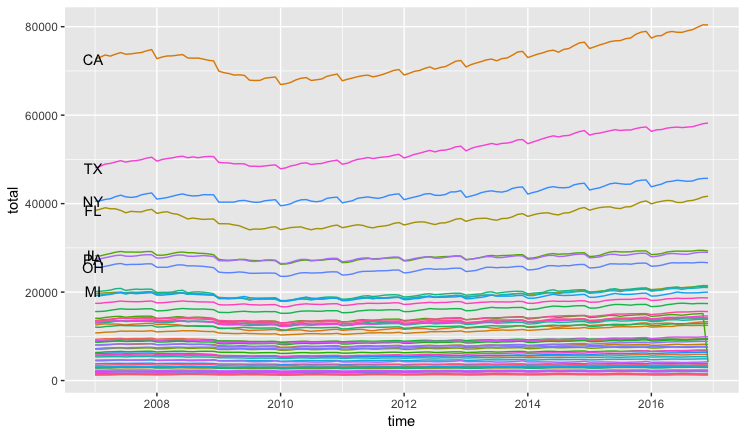
\includegraphics[width=.9\linewidth]{./employee_state.png}
\end{itemize}
\section{Technical Summary}
\label{sec-3}
\section{Appendix}
\label{sec-4}
% Emacs 24.5.1 (Org mode 8.2.10)
\end{document}
